\documentclass[a4wide,12pt]{article}
\usepackage{a4wide}
\usepackage[utf8]{inputenc}
\usepackage[english]{babel} 
\usepackage{url}

\usepackage{color}
\usepackage{graphicx}
\DeclareGraphicsExtensions{.jpg,.mps,.pdf,.png,.gif}
\usepackage{fancyvrb}
\usepackage{amsmath}
\usepackage{amsthm}
\usepackage{amssymb}
\usepackage{amsfonts}
\usepackage{listings}

\usepackage{tabularx,colortbl,booktabs}

\usepackage{pgf,tikz,pgfkeys,pgfplots}
\usetikzlibrary{shapes}
\usetikzlibrary{calc}
\usetikzlibrary{matrix}
\usetikzlibrary{positioning,shapes,shadows,arrows}

\usepackage[pdftex,
    bookmarks         = true,
    bookmarksnumbered = true,
    pdfpagemode       = None,
    pdfstartview      = FitH,
    pdfpagelayout     = SinglePage,
    colorlinks        = false,
    urlcolor          = blue,
    pdfborder         = {0 0 0}
    ]{hyperref}

\usepackage{pgf,tikz,pgfkeys,pgfplots}
\usetikzlibrary{shapes}
\usetikzlibrary{calc}
\usetikzlibrary{matrix}
\usetikzlibrary{positioning,shapes,shadows,arrows}


\hypersetup{
    pdfauthor   = {Deniz Aydin, Ivan Slijepcevic},
    pdftitle    = {report},
    pdfcreator  = {PDFLaTeX}
    pdfproducer = {PDFLaTeX}
}

\hypersetup{colorlinks,
            citecolor=red,
            filecolor=black,
            linkcolor=red,
            urlcolor=blue}


\date{18 November 2013}

\title{
Unsupervised and reinforcement learning in neural networks \\
Miniproject 1
}

\author{Deniz Aydin, Ivan Slijepcevic}

\definecolor{dkgreen}{rgb}{.13,.57,.33}
\definecolor{dkred}{rgb}{.57,.13,.33}


\begin{document}
\maketitle

\section{Scalability}

\subsection{Question (Paper \& Pencil)}     % subsection 1.1

\subsubsection{Constant input $x_o$ and threshold $\theta^*$}       % subsubsection 1.1.1
In the case of constant input and constant threshold ($x(t)=x_o$ and $\theta(t) = \theta^*$), the BCM learning rule has the form: 
\begin{equation}
\frac{d\omega_i}{dt} = \eta x_i(y^2-y\theta)= Aw^2-Bw
\end{equation}
where A and B are constants. Here, the main problem of this learning rule would be that the weights grow without bound, so they can not converge to stable values.  
\subsubsection{Stability of fixed points}
For the coupled differential equations: 

\begin{eqnarray}
\tau \dot \theta_M &=&  -\theta_M + y^p \\
\dot \omega &=& \eta x (y^2-y\theta) \\
\end{eqnarray}

we assume $\tau << \eta^{-1}$, so we can assume that $\theta$ converges much faster than $\omega$. At a fixed point for p=0, we would have: 

\begin{eqnarray}
\tau \dot \theta_M &=&  -\theta_M + y^p \\
0 &=& -\theta_M + y^p \\
\theta_M &=& 1
\end{eqnarray}
and 
\begin{eqnarray}
\dot \omega &=& \eta x (y^2-y) \\
\dot \omega &=& \eta x^2 \omega (\omega x- 1) \label{eq:p0}
\end{eqnarray}

so the fixed points are at $\omega = 0$ and $\omega = 1/x$. Fig. \ref{fig:p0} shows the plot of $\dot \omega$ for p=0, with the only stable fixed point being $\omega = 0$. 

\begin{figure}[h]
\centering
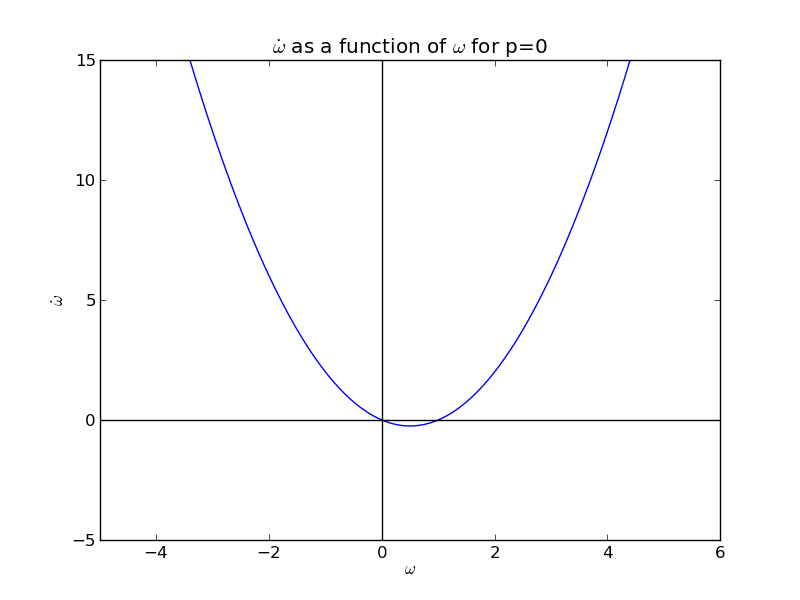
\includegraphics[width=0.7\textwidth]{./p0.png}
\caption{Fixed points of $\dot \omega$ are $\omega = 0$ and $\omega = 1/x$, as shown in figure. (Eq. \ref{eq:p0}). For simplicity we assume x=1.}
\label{fig:p0}
\end{figure}

For p=1, the coupled ODE's look like: 

\begin{eqnarray}
\tau \dot \theta_M &=&  -\theta_M + y \\
\theta_M &=& y
\end{eqnarray}
which leads to
\begin{eqnarray}
\dot \omega &=& \eta x (y^2-y^2) \\
\dot \omega &=& 0 \label{eq:p1}
\end{eqnarray}

and since the Eq. \ref{eq:p1} is zero everywhere, the system has either already converged or it is trivial, so we cannot discuss its stability as a function of $\omega$.

For p=2, the coupled ODE's are: 

\begin{eqnarray}
\theta_M &=& y^2
\end{eqnarray}

which leads to
\begin{eqnarray}
\dot \omega &=& \eta x (y^2-y^3) \\
\dot \omega &=&  \eta x^3w^2(1-wx) \label{eq:p2}
\end{eqnarray}

so the fixed points are at $\omega = 0$ and $\omega = 1/x$ once again. The only stable fixed point is $\omega = 1/x$ in this case, as can be seen from Fig. \ref{fig:p2}. 

\begin{figure}[h]
\centering
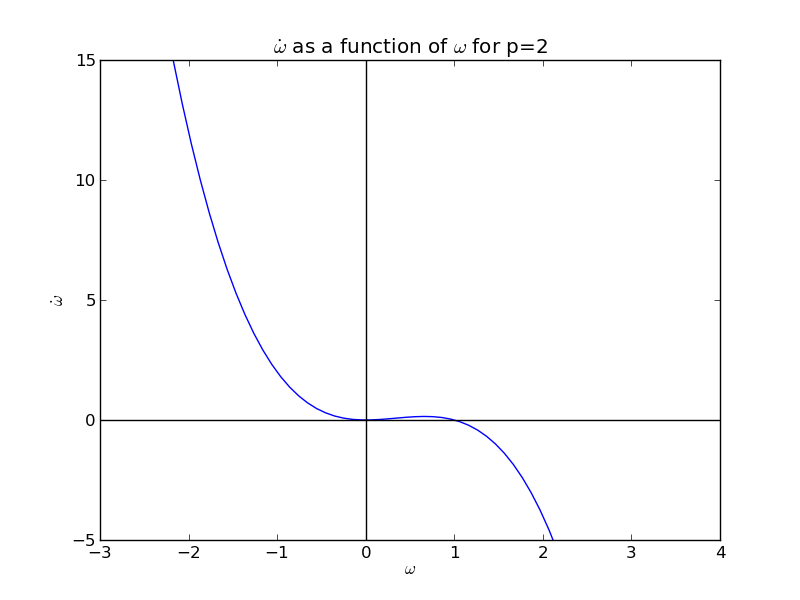
\includegraphics[width=0.7\textwidth]{./p2.png}
\caption{Fixed points of $\dot \omega$ are $\omega = 0$ and $\omega = 1/x$, as shown in figure. (Eq. \ref{eq:p2}, x=1).}
\label{fig:p2}
\end{figure}

For p=3, the coupled ODE's are: 

\begin{eqnarray}
\theta_M &=& y^3
\end{eqnarray}

which leads to
\begin{eqnarray}
\dot \omega &=& \eta x (y^2-y^4) \\
\dot \omega &=&  \eta x^3w^2(1-x^2w^2) \label{eq:p3}
\end{eqnarray}

so the fixed points are at $\omega = 0$ and $\omega = \pm 1/x$. The only stable fixed point is $\omega = 1/x$ again, seen in Fig. \ref{fig:p3}.

\begin{figure}[h]
\centering
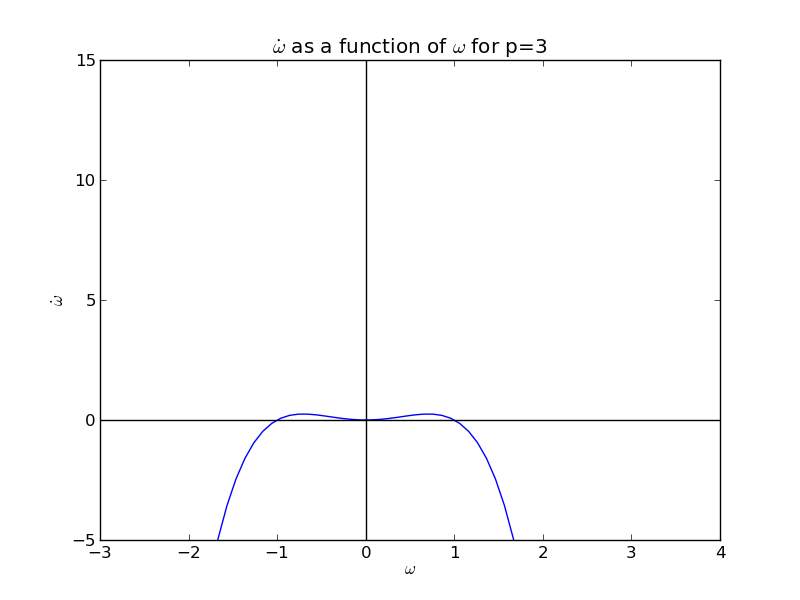
\includegraphics[width=0.7\textwidth]{./p3.png}
\caption{Fixed points of $\dot \omega$ are $\omega = 0$ and $\omega = \pm 1/x$, as shown in figure. (Eq. \ref{eq:p3}, x=1).}
\label{fig:p3}
\end{figure}
\newpage
For p=4, the coupled ODE's are: 

\begin{eqnarray}
\theta_M &=& y^4
\end{eqnarray}

which leads to
\begin{eqnarray}
\dot \omega &=& \eta x (y^2-y^5) \\
\dot \omega &=&  \eta x^3w^2(1-x^3w^3) \label{eq:p4}
\end{eqnarray}

so the fixed points are at $\omega = 0$ and $\omega =  1/x$. Fig. \ref{fig:p4} shows the stability of fixed points for this system, where the only stable fixed point is $\omega = 1/x$ once again.

\begin{figure}[h]
\centering
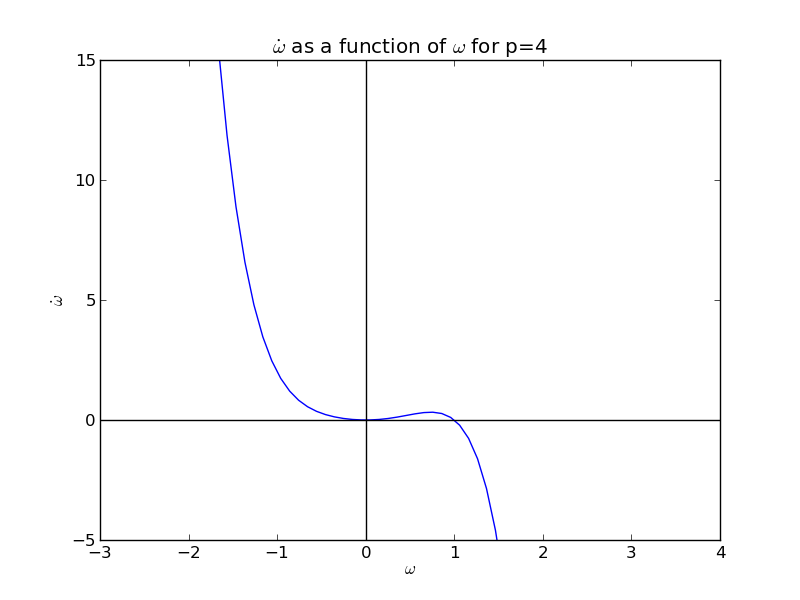
\includegraphics[width=0.7\textwidth]{./p4.png}
\caption{Fixed points of $\dot \omega$ are $\omega = 0$ and $\omega =  1/x$, as shown in figure. (Eq. \ref{eq:p4}, x=1).}
\label{fig:p4}
\end{figure}

We notice from the above examples that we can generalize stability of the fixed points for any $\theta_M = y^p$:
\begin{eqnarray}
\dot \omega &=& \eta x (y^2-y^{p+1}) \\
\dot \omega &=&  \eta x(x^2w^2-x^{p+1}w^{p+1}) \label{eq:general1}
\end{eqnarray}

and taking the derivative of $\dot \omega$ with respect to $\omega$ yields
\begin{eqnarray}
\frac{d\dot \omega}{d\omega} &=& \eta x (2x^2\omega-(p+1)x^{p+1}\omega^p) \label{eq:stab}
\end{eqnarray}

we know that the stability condition for fixed points should satisfy $\frac{d\dot \omega}{d\omega} <0$, so we can see from Eq. \ref{eq:stab} that when  $\omega = 1/x$:
\begin{eqnarray}
\frac{d\dot \omega}{d\omega} &=& \eta x (2x-(p+1)x)  \label{eq:ome}
\end{eqnarray}

and Eq. \ref{eq:ome} is always less than zero for $p > 1$. However, for $\omega = 0$ we see that $\frac{d\dot \omega}{d\omega} <0$ (Eq. \ref{eq:stab}) holds only if p =0. 

Finally, $\omega = -1/x$ can satisfy the stability criteria $\frac{d\dot \omega}{d\omega} <0$ for $p < 1$, but it is not a fixed point for these p values.




\subsection{Question (Simulation)}     % subsection 1.2

\subsubsection{Code organization}

Code is organized in several files. The files are described below.
\begin{itemize}
    \item \texttt{ODE.py} contains the abstract class \texttt{ODE} which defines
        the interface for ordinary differential equations.
    \item \texttt{Integrator.py} contains the abstract class \texttt{Integrator}
        and its derived class \texttt{ForwardDifference} which numerically solve
        an ordinary differential equation.
    \item \texttt{BCM.py} contains the class \texttt{BCM}, which derives from
        \texttt{ODE}. It implements the functionality of a BCM neuron, and also
        can be treated as an ODE.
    \item \texttt{main.py} runs the simulation for varying values of parameter
        $z$.
    \item \texttt{plotter.py} contains the various functionality for plotting.
        It can also be called as a script to plot the simulated data.
    \item \texttt{simulation.sh} is a script that runs the main simulation
        several times and then calls the plotter.
\end{itemize}


\subsubsection{Comment on results}

\begin{figure}[h]
\centering
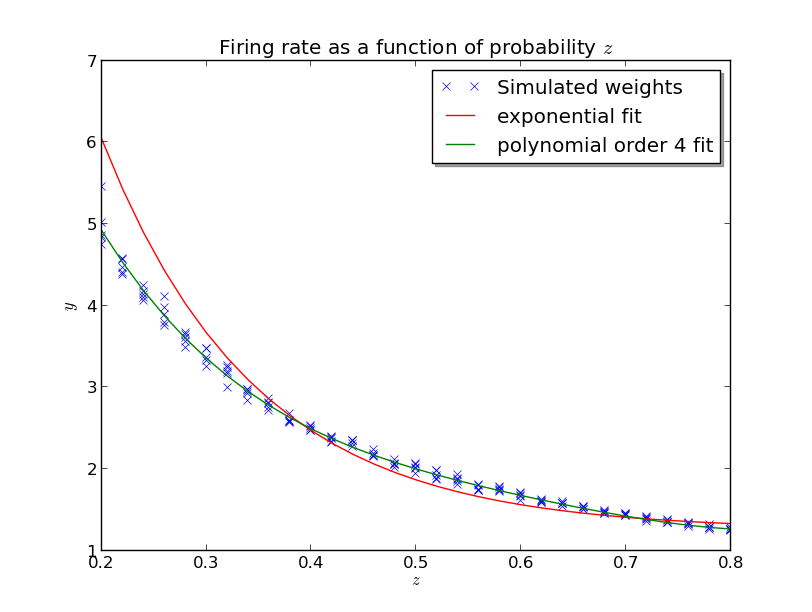
\includegraphics[width=0.7\textwidth]{figures/ex1-2.png}
\caption{Plot of a firing rate as a function of probability $z$, data from $5$
simulations, together with exponential and polynomial curve fits.}
\label{fig:ex12}
\end{figure}

The requested results can be seen in the Figure \ref{fig:ex12}. It can be
observed that neuron's response decays with probability $z$ as a $4$-th order
polynomial. This means, the more the input neuron fires, the connection between
them becomes weaker. From this we can assume that the BCM learning rule is
anti-Hebbian. In other words, $\theta$ is superlinear function of $y$, which
makes the expression $x(y^2 - y\theta)$ negative, and confirms the
anti-Hebbian learning.

\section{Selectivity and Optimization Principle}

\section{Explaining V1 Receptive Field Formation}

\paragraph{Preprocessing}
Normalization and generation of input patches was done in a separate
preprocessing step. Preprocessing is called with
%\begin{lstlisting}[language=bash]
%$ python preprocess.py
%\end{lstlisting}
Normalization step creates the file with suffix \texttt{\_normalized.data},
which contains a \texttt{numpy} array of normalized input image, serialized to
string. Afterwards, the file which describes patches is created. Its suffix is
\texttt{\_patches.data}. It contains $5000$ rows, where each row has the pixel
coordinates of upper-left corner of the $16 \times 16$ pixel patch. No two
patches are identical. This way of describing patches makes sure that additional
preprocessed data won't take too much memory, while still being easy to create
generated patches.

\begin{figure}[h]
\centering
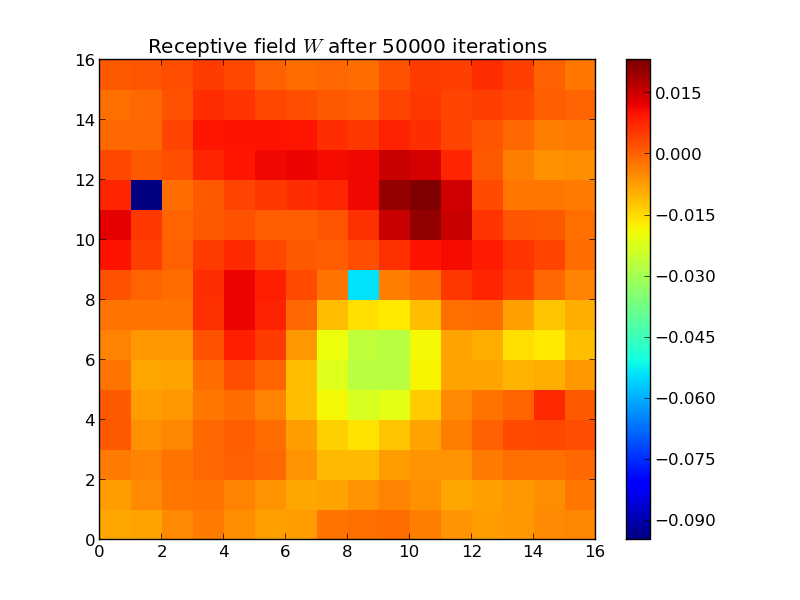
\includegraphics[width=0.7\textwidth]{../ex3/results1/img06}
\caption{}
\label{fig:img06}
\end{figure}

\begin{figure}[h]
\centering
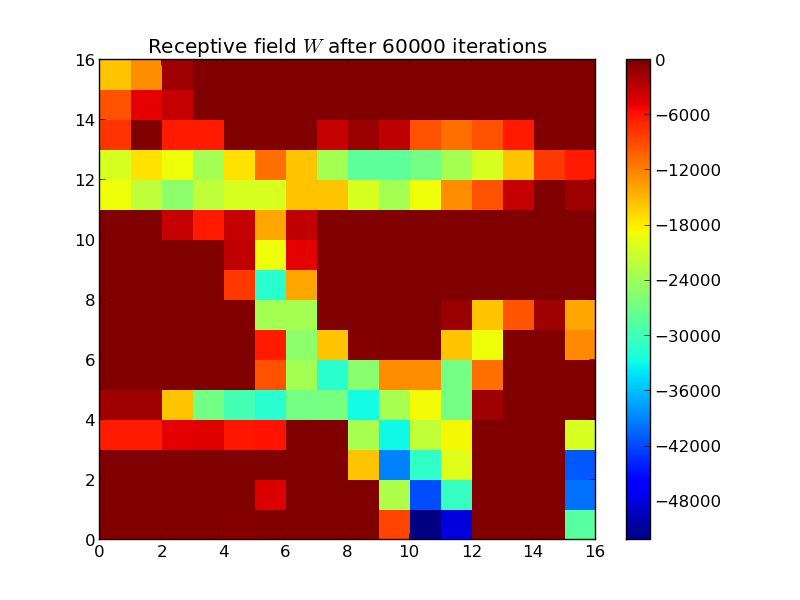
\includegraphics[width=0.7\textwidth]{../ex3/results1/img07}
\caption{}
\label{fig:img07}
\end{figure}

\begin{figure}[h]
\centering
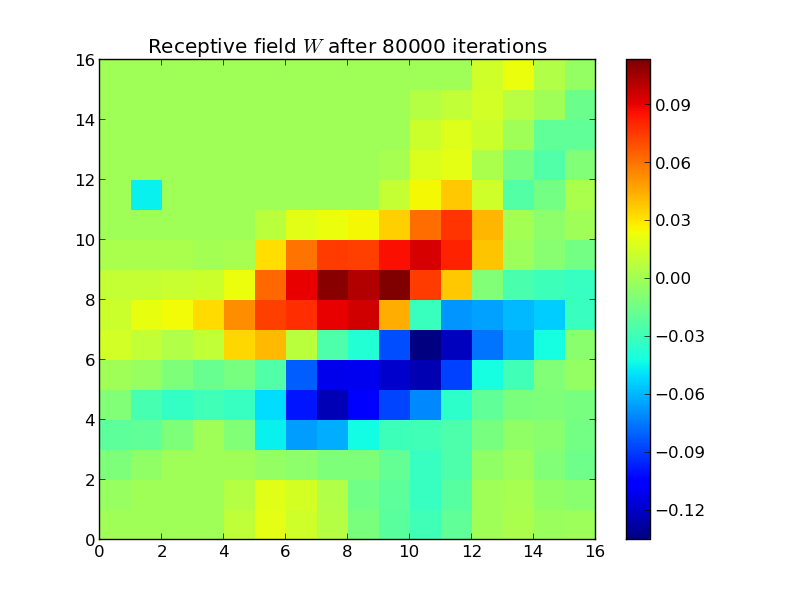
\includegraphics[width=0.7\textwidth]{../ex3/results1/img09}
\caption{}
\label{fig:img09}
\end{figure}

\begin{figure}[h]
\centering
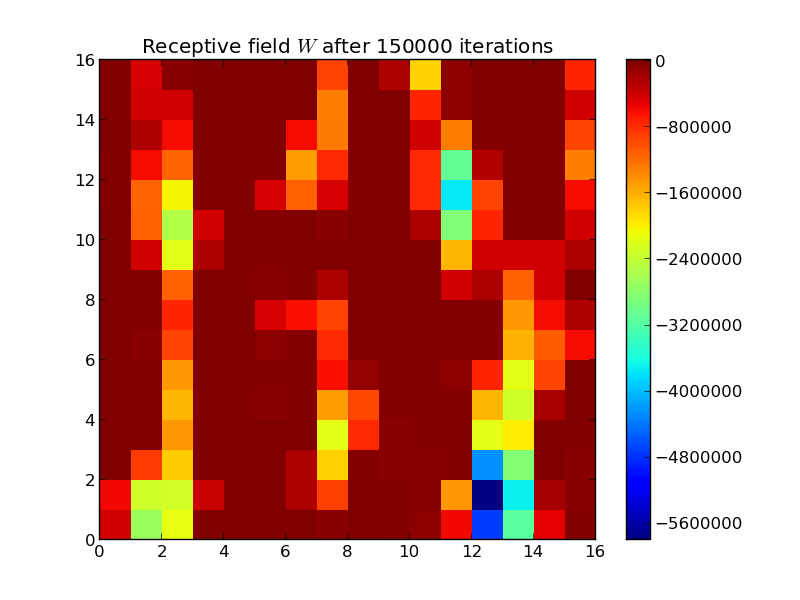
\includegraphics[width=0.7\textwidth]{../ex3/results1/img16}
\caption{}
\label{fig:img16}
\end{figure}

\begin{figure}[h]
\centering
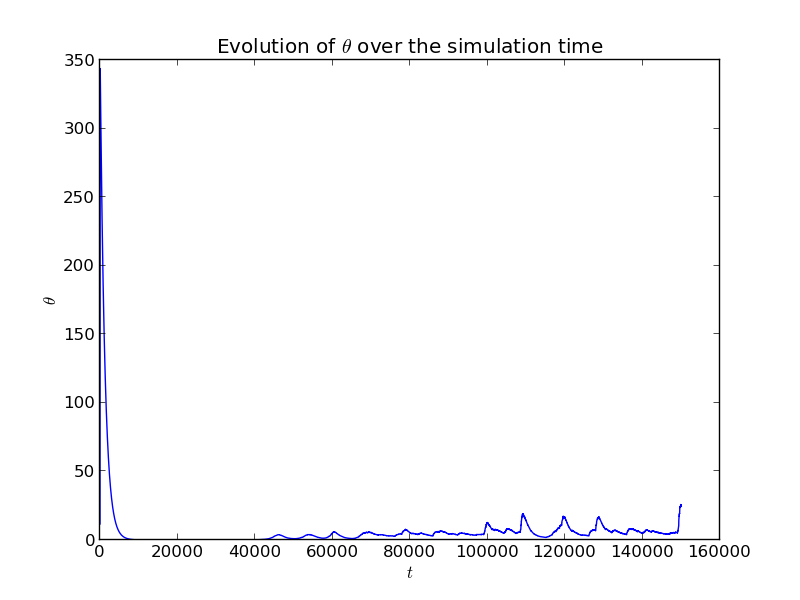
\includegraphics[width=0.7\textwidth]{../ex3/results1/theta}
\caption{}
\label{fig:theta}
\end{figure}

\paragraph{Simulation}
The simulation was done many times. Every simulation was done with $150000$
iterations, with $50000$ different patches. Every simulation has had different
permutations of patches, and occasionally, patches were constructed again using
preprocessing. Figures (mention them) show the typical development of a
receptive field. In the beginning--there is usually an initialization period, no
visible pattern. Then some lines start to emerge. In the end it is clearly
visible something similar to the Gabor filter. (need to comment this more
extensively)


\end{document}
